% ============================================================
%  AutoPipeAD: Automatic Selection of Preprocessing
%  Pipelines for Anomaly Detection in Images
%  Technical Article — English translation
%  Instituto Tecnológico de Costa Rica
%  IEEE Conference format
% ============================================================
\documentclass[conference]{IEEEtran}

% ----- Encoding and language -----
\usepackage[utf8]{inputenc}
\usepackage[T1]{fontenc}
\usepackage[english]{babel}

% ----- Mathematics -----
\usepackage{amsmath}
\usepackage{amssymb}

% ----- Tables and figures -----
\usepackage{graphicx}
\usepackage{booktabs}
\usepackage{array}
\usepackage{multirow}

% ----- References and URLs -----
\usepackage{url}
\usepackage{cite}

% ----- Typography -----
\usepackage{microtype}

% ----- Source code -----
\usepackage{listings}
\lstset{
    basicstyle=\scriptsize\ttfamily,
    breaklines=true,
    breakatwhitespace=false,
    columns=flexible,
    keepspaces=true,
    showstringspaces=false,
    aboveskip=4pt,
    belowskip=2pt,
}

% ----- TikZ diagrams -----
\usepackage{xcolor}
\usepackage{tikz}
\usetikzlibrary{shapes.geometric, arrows.meta, positioning, fit, backgrounds, calc}

% ----- Hyperlinks (loaded last for IEEEtran compatibility) -----
\usepackage[hidelinks,breaklinks]{hyperref}

% ============================================================
%  COLORS
% ============================================================
\definecolor{tecblue}{RGB}{0,51,102}
\definecolor{lightblue}{RGB}{210,230,255}
\definecolor{lightgreen}{RGB}{210,240,220}
\definecolor{lightyellow}{RGB}{255,250,210}
\definecolor{lightgray}{RGB}{240,240,240}
\definecolor{lightred}{RGB}{255,220,220}

% ============================================================
%  TIKZ STYLES
% ============================================================
\tikzstyle{modulo}   = [rectangle, rounded corners=3pt, minimum width=2.2cm,
    minimum height=0.85cm, text centered, draw=tecblue, fill=lightblue,
    font=\scriptsize\bfseries, text width=2.0cm]
\tikzstyle{externo}  = [rectangle, minimum width=2.0cm,
    minimum height=0.85cm, text centered, draw=gray, fill=lightgray,
    font=\scriptsize, text width=1.85cm, dashed]
\tikzstyle{actor}    = [rectangle, minimum width=2.0cm,
    minimum height=0.85cm, text centered, draw=tecblue, fill=lightyellow,
    font=\scriptsize, text width=1.85cm]
\tikzstyle{estado}   = [rectangle, rounded corners=4pt, minimum width=2.6cm,
    minimum height=0.8cm, text centered, draw=tecblue, fill=lightgreen,
    font=\scriptsize, text width=2.4cm]
\tikzstyle{decision} = [diamond, aspect=2.2, minimum width=2.2cm,
    minimum height=0.7cm, text centered, draw=tecblue, fill=lightyellow,
    font=\scriptsize, text width=2.0cm]
\tikzstyle{startend} = [circle, minimum size=0.5cm, draw=tecblue, fill=tecblue]
\tikzstyle{iface}    = [rectangle, rounded corners=2pt, minimum width=2.2cm,
    minimum height=0.85cm, text centered, draw=tecblue!60, fill=lightred,
    font=\scriptsize\itshape, text width=2.0cm]
\tikzstyle{flecha}      = [-{Stealth[length=5pt]}, thick, color=tecblue]
\tikzstyle{flechadash}  = [-{Stealth[length=5pt]}, dashed, color=gray]
\tikzstyle{flechaopc}   = [-{Stealth[length=5pt]}, dotted, thick, color=tecblue!60]

% ============================================================
%  PDF METADATA
% ============================================================
\hypersetup{
    pdftitle={AutoPipeAD: Automatic Selection of Preprocessing Pipelines
              for Anomaly Detection in Images},
    pdfauthor={Ricardo Antonio Borbón Mena}
}

% ============================================================
\begin{document}

\title{AutoPipeAD: Automatic Selection of Preprocessing Pipelines
       for Anomaly Detection in Images}

\author{%
\IEEEauthorblockN{Ricardo Antonio Borbón Mena}
\IEEEauthorblockA{School of Computer Engineering\\
Instituto Tecnológico de Costa Rica\\
Cartago, Costa Rica\\
ricardobm@estudiantec.cr}
\and
\IEEEauthorblockN{Luis Alberto Chavarría Zamora (Advisor)}
\IEEEauthorblockA{School of Computer Engineering\\
Instituto Tecnológico de Costa Rica\\
Cartago, Costa Rica\\
lachavarria@itcr.ac.cr}
}

\maketitle

% ============================================================
%  ABSTRACT
% ============================================================
\begin{abstract}
Anomaly detection in images is a relevant problem in industrial inspection,
quality control, and medical analysis. The performance of anomaly detectors
depends largely on the preprocessing applied to the input images, and
manually choosing this chain of transformations is time-consuming and
requires specialized knowledge in computer vision. This work presents
AutoPipeAD, an open-source Python library that automates the search for the
optimal preprocessing pipeline for a user-provided base anomaly detection
model. The library receives image datasets organized into subdirectories of
normal and anomalous samples, and systematically evaluates combinations of
seven predefined transformations through exhaustive grid search or Bayesian
optimization with Optuna (TPE sampling and median pruning). Parallel
evaluation was implemented with joblib. The configurable metrics include
AUC-ROC, F1-score, precision, recall, and false positive rate; the winning
pipeline is saved in JSON or YAML to guarantee reproducibility. Experiments
with three synthetic datasets verified the correct functioning of the library
and its compatibility with scikit-learn and PyTorch base models.
\end{abstract}

\begin{IEEEkeywords}
anomaly detection, image preprocessing, automatic pipeline selection, grid
search, Bayesian optimization, Optuna, parallel processing, IsolationForest,
AUC-ROC, MVTec AD
\end{IEEEkeywords}

% ============================================================
%  I. INTRODUCTION
% ============================================================
\section{Introduction}

Anomaly detection in images consists of automatically identifying instances
that deviate from an expected pattern, called normal~\cite{chandola2009anomaly}.
Its applications range from defect inspection on industrial surfaces to
medical image analysis and visual surveillance. Unlike supervised
classification, anomaly detectors are usually trained assuming that anomalous
samples are scarce or unknown: the model learns the distribution of normal
cases and assigns an anomaly score to each new
instance~\cite{chandola2009anomaly}.

The performance of these detectors depends largely on the preprocessing
applied to the input images. Operations such as resizing, Gaussian smoothing,
statistical normalization, or adaptive histogram equalization change the
distribution of the image features, and can notably improve or worsen the
model's ability to distinguish normal from anomalous~\cite{gonzalez2018dip}.
Choosing this chain of transformations—the preprocessing pipeline—is usually
done manually, by trial and error, which is time-consuming and requires
experience in computer vision.

AutoPipeAD was developed to automate this process. The library receives an
image dataset and a base anomaly detection model compatible with the
scikit-learn or PyTorch interface, and automatically searches for the
combination of transformations that maximizes the model's performance on a
validation set.

The scope of the project is limited to the selection of the preprocessing
pipeline: it does not include training or optimizing the architecture of the
base model, nor multiclass classification, semantic segmentation, object
detection, graphical interface, or deployment as a web service.

% ============================================================
%  II. BACKGROUND
% ============================================================
\section{Background}

\subsection{Anomaly Detection in Images}

Chandola, Banerjee, and Kumar~\cite{chandola2009anomaly} conducted a broad
review of anomaly detection methods, classifying them according to the level
of supervision available. For images, the most widely used approach is
one-class learning: the model is trained only with normal samples and assigns
an anomaly score during inference.

The One-Class Support Vector Machine (One-Class SVM, OC-SVM) by
Schölkopf et al.~\cite{scholkopf2001ocsvm} estimates a hypersurface that
encloses the distribution of normal samples in the feature space. The
Isolation Forest by Liu, Ting, and Zhou~\cite{liu2012isolation} follows a
different idea: it isolates instances by building random decision trees, under
the assumption that anomalies are isolated with fewer partitions than normal
samples. Both models expose the scikit-learn fit/predict
interface~\cite{pedregosa2011sklearn}, which makes them natural candidates for
use with AutoPipeAD.

More recent methods, such as PaDiM~\cite{defard2021padim} and
PatchCore~\cite{roth2022patchcore}, leverage deep representations from
pretrained neural networks to detect anomalies in industrial images with high
precision, although their integration is more complex.

The MVTec AD dataset~\cite{bergmann2019mvtec} is the most widely used
benchmark for evaluating anomaly detection methods in industrial images. It
contains 15~categories of objects and textures with real defects, and was
used as a compatibility reference in this work.

\subsection{Image Preprocessing}

Gonzalez and Woods~\cite{gonzalez2018dip} described the fundamental
transformations of digital images. For anomaly detection, the most relevant
are:

\begin{itemize}
\item \textbf{Resizing}: standardizes image dimensions to ensure fixed-length
  feature vectors.
\item \textbf{Gaussian smoothing}: reduces high-frequency noise by convolving
  the image with a Gaussian kernel of standard deviation $\sigma$.
\item \textbf{Median filter}: removes impulsive noise (salt and pepper)
  without erasing the image edges.
\item \textbf{Statistical normalization}: centers and scales the intensity
  values according to the mean $\mu$ and standard deviation $\sigma$ of the
  channel, producing the transformed image $(I - \mu)/\sigma$.
\item \textbf{CLAHE} (Contrast Limited Adaptive Histogram
  Equalization): improves local contrast by dividing the image into
  blocks and applying histogram equalization with a clip limit that avoids
  amplifying noise.
\item \textbf{Gamma correction}: adjusts the global brightness through the
  power function $I_{\text{out}} = I_{\text{in}}^{\gamma}$, where
  $\gamma < 1$ brightens the image and $\gamma > 1$ darkens it.
\item \textbf{Grayscale conversion}: reduces the RGB image to a single
  luminance channel, lowering the dimensionality of the feature space.
\end{itemize}

There are no general guidelines for choosing the preprocessing pipeline in
anomaly detection: the optimal combination depends on the type of defect, the
lighting conditions, and the architecture of the base model.

\subsection{Automated Machine Learning and Pipeline Search}

Automated machine learning (AutoML) studies how to automatically select and
configure machine learning algorithms and pipelines~\cite{yang2020automl}. The
search for preprocessing pipelines is a subproblem of AutoML, where the search
space is defined by the available transformations and their hyperparameters,
whether discrete or continuous.

Exhaustive grid search evaluates the Cartesian product of all discrete
options. It guarantees exploring the entire space, but its complexity grows as
$O\!\left(\prod_{i=1}^{n} |S_i|\right)$, where $|S_i|$ is the number of options
of step $i$ of the pipeline~\cite{hastie2009elements}.

Bayesian optimization builds a probabilistic model of the objective function
and uses it to decide the next points to evaluate, converging with fewer
trials than random search~\cite{snoek2012practical}.
Optuna~\cite{akiba2019optuna} implements Tree-structured Parzen Estimator
(TPE) sampling together with the median pruner (MedianPruner), which discards
trials whose performance falls below the median of the study after a minimum
number of evaluations.

\subsection{Parallel Evaluation}

Since the evaluation of each candidate pipeline is independent of the others,
this task naturally lends itself to parallelism. The joblib library,
distributed together with scikit-learn~\cite{pedregosa2011sklearn}, offers a
high-level interface for process-based parallelism through the loky backend,
compatible with Windows, Linux, and macOS without needing to explicitly
protect the entry point in Python scripts. The efficiency of parallelization
is measured with the speedup, defined as the ratio
$T_{\text{seq}} / T_{\text{par}}$ between the sequential and parallel
execution times.

\subsection{Evaluation Metrics}

The evaluation of anomaly detectors is based on binary classification metrics.
Fawcett~\cite{fawcett2006roc} described the area under the ROC curve (AUC-ROC)
as the most robust metric for comparing detectors, because it does not depend
on the decision threshold or on class imbalance. AUC-ROC takes values between
0 and 1, where 1.0 indicates perfect classification and 0.5 corresponds to
random prediction. The F1-score, precision, and recall complement AUC-ROC by
considering a specific binarization threshold.

The CIFAR-10 dataset~\cite{krizhevsky2009cifar}, with 60\,000 images of
$32\times32$ pixels in ten categories, was used as a basis for building
one-vs-rest anomaly scenarios, a standard protocol for evaluating unsupervised
detectors on classification data.

% ============================================================
%  III. DESCRIPTION OF THE DEVELOPED SOLUTION
% ============================================================
\section{Description of the Developed Solution}

The AutoPipeAD repository, containing the complete implementation, the
documentation, and the usage examples, is available on GitHub at
\url{https://github.com/ItsRichard7/AutoPipeAD}.

\subsection{General Architecture}

AutoPipeAD was designed as a Python library with six modules and well-defined
public interfaces. Figure~\ref{fig:arquitectura} shows how data flows between
the system components.

\begin{figure*}[t]
\centering
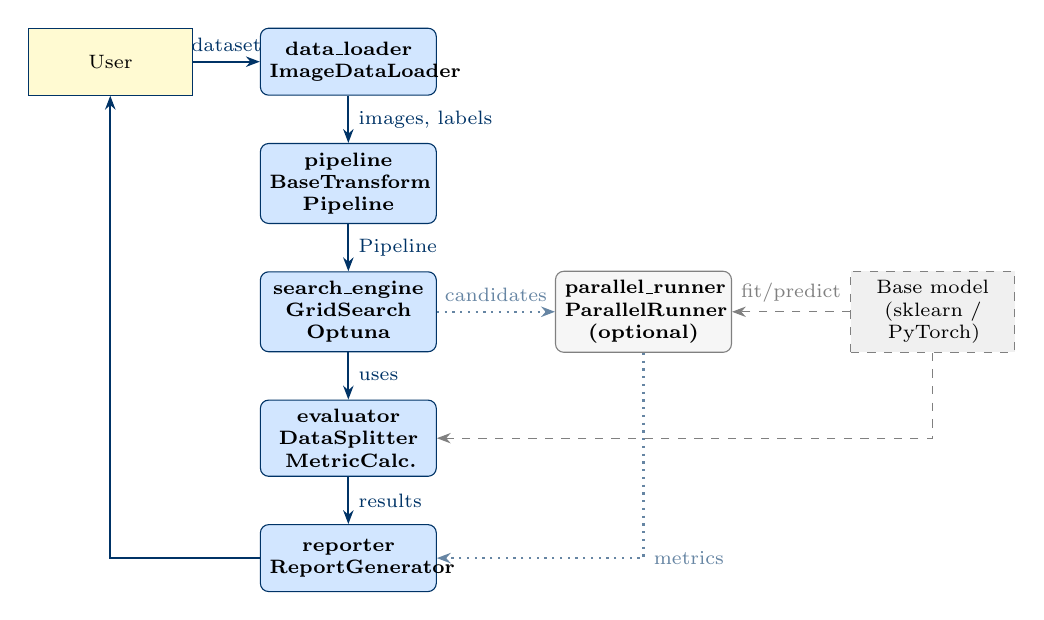
\begin{tikzpicture}[node distance=0.60cm and 0.80cm]

    %% --- Left column: external actors ---
    \node[actor]  (usr)    {User};

    %% --- Central column: main flow ---
    \node[modulo, right=0.85cm of usr]  (dl)  {data\_loader\\ImageDataLoader};
    \node[modulo, below=0.60cm of dl]   (pl)  {pipeline\\BaseTransform\\Pipeline};
    \node[modulo, below=0.60cm of pl]   (se)  {search\_engine\\GridSearch\\Optuna};
    \node[modulo, below=0.60cm of se]   (ev)  {evaluator\\DataSplitter\\MetricCalc.};
    \node[modulo, below=0.60cm of ev]   (rep) {reporter\\ReportGenerator};

    %% --- Optional branch: parallel_runner ---
    \node[modulo, right=1.5cm of se, fill=lightgray!60, draw=gray]
          (pr)  {parallel\_runner\\ParallelRunner\\(optional)};

    %% --- Base model (external actor) ---
    \node[externo, right=1.5cm of pr] (mb) {Base model\\(sklearn /\\PyTorch)};

    %% --- Main flow arrows ---
    \draw[flecha] (usr)  -- node[above, font=\scriptsize]{dataset} (dl);
    \draw[flecha] (dl)   -- node[right, font=\scriptsize]{images, labels} (pl);
    \draw[flecha] (pl)   -- node[right, font=\scriptsize]{Pipeline} (se);
    \draw[flecha] (se)   -- node[right, font=\scriptsize]{uses} (ev);
    \draw[flecha] (ev)   -- node[right, font=\scriptsize]{results} (rep);
    \draw[flecha] (rep.west) -| (usr.south);

    %% --- Optional branch ---
    \draw[flechaopc] (se.east) -- node[above, font=\scriptsize]{candidates} (pr.west);
    \draw[flechaopc] (pr.south) |- node[right, font=\scriptsize]{metrics} (rep.east);

    %% --- Base model → modules ---
    \draw[flechadash] (mb) -- node[above, font=\scriptsize]{fit/predict} (pr);
    \draw[flechadash] (mb.south) |- (ev.east);

\end{tikzpicture}
\caption{Architecture of AutoPipeAD. Solid arrows correspond to the main
  automatic search flow; dotted arrows indicate the \texttt{parallel\_runner}
  module, an independent and optional component.}
\label{fig:arquitectura}
\end{figure*}

\subsection{Data Loading Module (\texttt{data\_loader})}

The ImageDataLoader class loaded images from a root directory that had to
contain the \texttt{normal/} (label 0) and \texttt{anomaly/} (label 1)
subdirectories. The \texttt{.png}, \texttt{.jpg}, and \texttt{.bmp} formats
were supported; files with an unsupported extension were skipped with a
logging warning. The load() method returned a dense NumPy array of shape
$(n, H, W, C)$ if all images shared dimensions, or an object array otherwise.

\subsection{Transformations Module (\texttt{pipeline})}

\subsubsection{Base class \texttt{BaseTransform}}

All transformations inherit from the abstract class \texttt{BaseTransform},
which defines two mandatory methods:

\begin{lstlisting}[language=Python]
class BaseTransform(ABC):
    @abstractmethod
    def apply(self, image: np.ndarray) -> np.ndarray:
        ...
    @abstractmethod
    def get_params(self) -> dict:
        ...
\end{lstlisting}

This contract allows the search engine to treat any transformation uniformly.
Figure~\ref{fig:clases} shows the class hierarchy of the transformations
module.

\begin{figure*}[t]
\centering
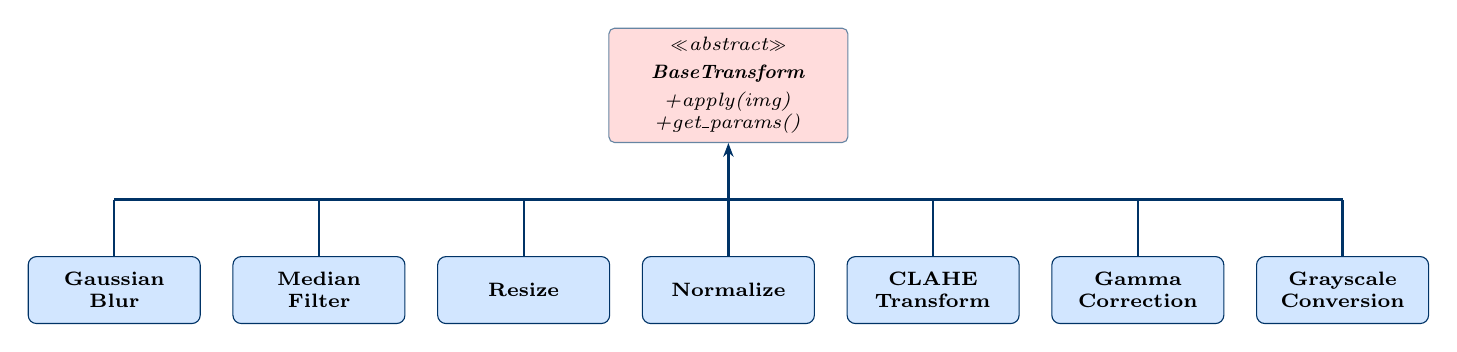
\begin{tikzpicture}

    %% Base class centered
    \node[iface, minimum width=3.0cm, text width=2.8cm] at (0,0) (bt)
          {\textit{\guillemotleft{}abstract\guillemotright{}}\\[2pt]
           \textbf{BaseTransform}\\[2pt]
           +apply(img)\\+get\_params()};

    %% Seven concrete classes, equidistant 2.6cm between centers
    \node[modulo, text width=1.95cm, minimum width=2.1cm] at (-7.8,-2.6) (gb)
          {Gaussian\\Blur};
    \node[modulo, text width=1.95cm, minimum width=2.1cm] at (-5.2,-2.6) (mf)
          {Median\\Filter};
    \node[modulo, text width=1.95cm, minimum width=2.1cm] at (-2.6,-2.6) (rs)
          {Resize};
    \node[modulo, text width=1.95cm, minimum width=2.1cm] at ( 0.0,-2.6) (nm)
          {Normalize};
    \node[modulo, text width=1.95cm, minimum width=2.1cm] at ( 2.6,-2.6) (cl)
          {CLAHE\\Transform};
    \node[modulo, text width=1.95cm, minimum width=2.1cm] at ( 5.2,-2.6) (gc)
          {Gamma\\Correction};
    \node[modulo, text width=1.95cm, minimum width=2.1cm] at ( 7.8,-2.6) (gs)
          {Grayscale\\Conversion};

    %% Horizontal collector bar (UML bus style)
    \draw[thick, color=tecblue] (-7.8,-1.45) -- (7.8,-1.45);

    %% Inheritance arrow: bar → BaseTransform (points to the parent)
    \draw[flecha] (0,-1.45) -- (bt.south);

    %% Vertical stubs: top of each node → bar
    \draw[thick, color=tecblue] (gb.north) -- (-7.8,-1.45);
    \draw[thick, color=tecblue] (mf.north) -- (-5.2,-1.45);
    \draw[thick, color=tecblue] (rs.north) -- (-2.6,-1.45);
    \draw[thick, color=tecblue] (nm.north) -- ( 0.0,-1.45);
    \draw[thick, color=tecblue] (cl.north) -- ( 2.6,-1.45);
    \draw[thick, color=tecblue] (gc.north) -- ( 5.2,-1.45);
    \draw[thick, color=tecblue] (gs.north) -- ( 7.8,-1.45);

\end{tikzpicture}
\caption{Class hierarchy of the \texttt{pipeline} module. The seven concrete
  transformations inherited directly from \texttt{BaseTransform} and
  implemented \texttt{apply()} and \texttt{get\_params()}.
  The collector bar represents the inheritance of the several subclasses from
  a single parent.}
\label{fig:clases}
\end{figure*}

\subsubsection{Predefined transformations}

The library implements seven transformations: GaussianBlur (Gaussian smoothing
with a square kernel of positive odd size), MedianFilter (median filter,
$\text{kernel} \geq 3$), Normalize (normalization by mean and standard
deviation, produces float32), Resize (bilinear resizing with OpenCV),
CLAHETransform (applies CLAHE to the $L$ channel of the LAB space in color
images, or directly on grayscale images), GammaCorrection (implemented with a
lookup table for integer images), and GrayscaleConversion (RGB to grayscale
conversion).

\subsubsection{\texttt{Pipeline} class}

The \texttt{Pipeline} class composes an ordered sequence of
\texttt{BaseTransform} instances. It applies each transformation in order, and
returns a dictionary with a \{index\}\_\{Class\} key per step, which allows
serializing the winning configuration.

\subsection{Search Module (\texttt{search\_engine})}

The search space is expressed as a Python dictionary where each key identifies
a pipeline step and the value is a list of candidate transformations. A real
usage example with \texttt{val\_size=0.3}:

\begin{lstlisting}[language=Python]
search_space = {
    "resize":    [Resize(width=32, height=32)],
    "blur":      [GaussianBlur(kernel_size=3),
                  GaussianBlur(kernel_size=5)],
    "normalize": [Normalize(mean=0.5, std=0.5)],
}
engine = GridSearchEngine(
    search_space, val_size=0.3, random_state=42)
best, metrics, results = engine.run(
    images, labels,
    base_model=IsolationForest(
        contamination=0.2, random_state=0),
    metric="auc_roc")
\end{lstlisting}

For each step of the space, both engines automatically and transparently add
the option of omitting it: the user configures nothing additional and the
search also evaluates pipelines without that transformation. An omitted step
simply does not appear in the resulting pipeline nor in its serialized
configuration, which preserves the type contract of \texttt{BaseTransform} and
makes reconstruction trivial.

\subsubsection{GridSearchEngine}

It generates the Cartesian product of the candidate lists, extended with the
per-step omission option, and evaluates each combination exhaustively; the
effective space is $\prod_{i=1}^{n} (|S_i|+1)$ combinations. For each candidate
pipeline: (1)~the sequence of transformations is applied to each image and the
result is flattened into a feature vector; (2)~a deep copy of the base model is
trained on the training subset; (3)~the metrics are computed on the stratified
validation subset. The objective value is compared according to the direction
of the metric: false\_positive\_rate is minimized, the rest are maximized. The
automatically generated candidates that cannot be evaluated (for example,
omitting resizing with images of heterogeneous dimensions) are recorded with
NaN metrics and a warning, without aborting the search; a NaN candidate never
becomes the winner.

\subsubsection{OptunaSearchEngine}

It implements Bayesian optimization with TPESampler (fixed seed) and
MedianPruner~\cite{akiba2019optuna}. It accepts the same search space format as
GridSearchEngine and exposes the same signature; the omission of each step is
modeled as an additional categorical index in the sampler. The NaN values
produced by trials with a single class in the validation set (or by
unevaluable candidates) are replaced with $\pm\infty$ so as not to corrupt the
Optuna study.

\subsection{Evaluation Module (\texttt{evaluator})}

\subsubsection{DataSplitter}

It generates stratified train/val partitions from
scikit-learn~\cite{pedregosa2011sklearn}. Stratification ensures that the
proportion of anomalous samples is equivalent in both subsets, which is
important in imbalanced datasets. It also supports $k$-fold cross-validation.
The splitter configuration can be saved and reloaded in JSON or YAML.

\subsubsection{MetricCalculator}

It computes AUC-ROC, F1-score, precision, recall, and false positive rate. To
obtain the continuous scores required by AUC-ROC, the predict\_proba,
score\_samples (negated), and decision\_function (negated) methods of the base
model are tried in order. The IsolationForest predictions (convention
$-1$=anomaly, $+1$=normal) are normalized to $\{0, 1\}$ labels.

\subsection{Parallel Execution Module (\texttt{parallel\_runner})}

The \texttt{ParallelRunner} class evaluates a list of pipelines concurrently.
Each process evaluates a pipeline on an independent copy of the base model,
with no mutable shared state. The benchmark() method measures the speedup as
$T_{\text{seq}} / T_{\text{par}}$, and verifies that the parallel and
sequential results are numerically equivalent.

\subsection{Reporting Module (\texttt{reporter})}

The \texttt{ReportGenerator} class always produces an HTML report, with
optional PDF export. If the binary is not available, the system logs a warning
and keeps the HTML (graceful degradation). The charts are generated with
matplotlib and embedded as base64 data URIs, producing a self-contained HTML
document. The winning pipeline configuration is saved in JSON with the
structure:
\begin{lstlisting}
{
  "0_Resize":       {"width": 32, "height": 32},
  "1_GaussianBlur": {"kernel_size": 3},
  "2_Normalize":    {"mean": 0.5, "std": 0.5}
}
\end{lstlisting}
The static method rebuild\_pipeline(config) reconstructs the pipeline from this
file, which allows repeating exactly the same execution; the steps omitted by
the search do not appear in the configuration and the indices of the present
ones remain contiguous.

If the user does not configure an output directory, the files are written to a
reports/ subfolder next to the script that invokes the library; in interactive
sessions (Jupyter) the working directory is used, which matches that of the
notebook. The folder is created automatically, so the standard use case does
not require configuring paths.

\subsection{Pipeline Evaluation Flow}

Figure~\ref{fig:flujo} shows the activity diagram of the evaluation process of
a candidate pipeline within the search engine.

\begin{figure}[t]
\centering
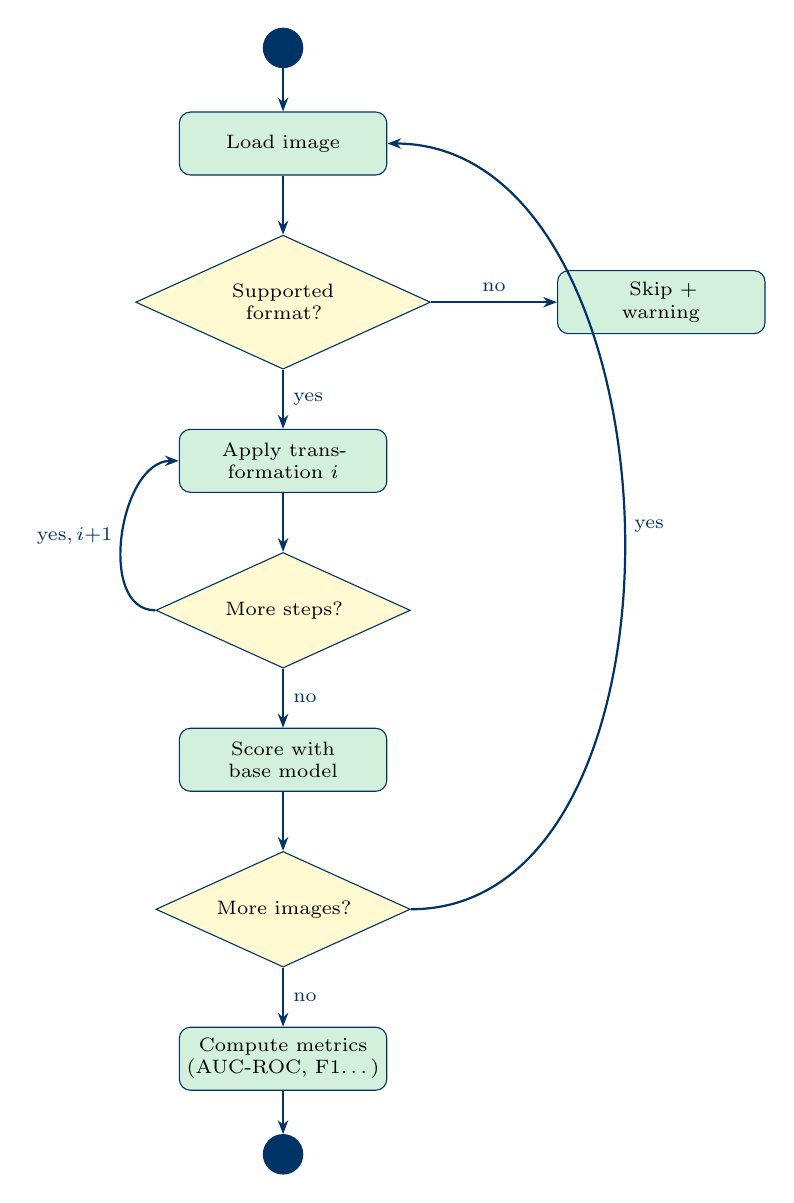
\begin{tikzpicture}[node distance=0.75cm]
    \node[startend] (ini)    {};
    \node[estado,   below=0.55cm of ini] (load)   {Load image};
    \node[decision, below=of load]        (valid)  {\scriptsize Supported format?};
    \node[estado,   right=1.6cm of valid] (omit)   {Skip +\\warning};
    \node[estado,   below=of valid]       (trans)  {Apply transformation $i$};
    \node[decision, below=of trans]       (more)   {\scriptsize More steps?};
    \node[estado,   below=of more]        (score)  {Score with\\base model};
    \node[decision, below=of score]       (imgs)   {\scriptsize More images?};
    \node[estado,   below=of imgs]        (metric) {Compute metrics\\(AUC-ROC, F1\ldots)};
    \node[startend, below=0.55cm of metric] (fin)  {};

    \draw[flecha] (ini)    -- (load);
    \draw[flecha] (load)   -- (valid);
    \draw[flecha] (valid)  -- node[right, font=\scriptsize]{yes} (trans);
    \draw[flecha] (valid)  -- node[above, font=\scriptsize]{no} (omit);
    \draw[flecha] (trans)  -- (more);
    \draw[flecha] (more.west) to[out=180,in=180]
                 node[left, font=\scriptsize]{yes,\,$i{+}1$} (trans.west);
    \draw[flecha] (more)   -- node[right, font=\scriptsize]{no} (score);
    \draw[flecha] (score)  -- (imgs);
    \draw[flecha] (imgs.east) to[out=0,in=0]
                 node[right, font=\scriptsize]{yes} (load.east);
    \draw[flecha] (imgs)   -- node[right, font=\scriptsize]{no} (metric);
    \draw[flecha] (metric) -- (fin);
\end{tikzpicture}
\caption{Activity diagram of the evaluation of a candidate pipeline.
  This flow was executed for each combination generated by the search engine.}
\label{fig:flujo}
\end{figure}

\subsection{Design Decisions}

Base model injection: the search engine receives the base model as an argument
and clones it before each evaluation. This ensures that all candidates are
evaluated on an identical untrained model, preserving comparability and
reproducibility.

Module-level functions for shared logic: the \texttt{evaluate\_pipeline()},
\texttt{is\_better()} and \texttt{validate\_metric()} functions were defined at
the module level, so that \texttt{GridSearchEngine}, \texttt{OptunaSearchEngine}
and \texttt{ParallelRunner} could use them without needing inheritance.

Choice of joblib over multiprocessing: joblib was chosen because it abstracts
the differences between platforms (fork model on Linux versus spawn on
Windows), is compatible with both search engines, and is the same dependency
used by scikit-learn~\cite{pedregosa2011sklearn}.

Choice of Jinja2 + pdfkit: WeasyPrint was discarded because it requires the GTK
graphics stack (Pango/Cairo), not available on Windows without complex
configuration. Instead, pdfkit was adopted with fault tolerance.

Step omission by absence: the omitted step was chosen to be represented as
absence (it does not appear in the pipeline nor in its serialized
configuration) instead of an explicit marker or an identity transformation:
this preserves the type contract of \texttt{BaseTransform} and reconstruction
from JSON/YAML works without special cases, including the empty pipeline.

\subsection{Technologies Used}

Table~\ref{tab:tecnologias} summarizes the main dependencies.

\begin{table}[t]
\centering
\renewcommand{\arraystretch}{1.2}
\caption{Main dependencies of AutoPipeAD.}
\label{tab:tecnologias}
\begin{tabular}{@{}lll@{}}
\toprule
\textbf{Component} & \textbf{Library} & \textbf{Minimum version} \\
\midrule
Image processing          & OpenCV        & 4.9  \\
                          & scikit-image  & 0.22 \\
                          & Pillow        & 10.0 \\
Numerical computing       & NumPy         & 1.26 \\
ML models and interface   & scikit-learn  & 1.4  \\
                          & PyTorch       & 2.2  \\
Bayesian search           & Optuna        & 3.6  \\
Parallelism               & joblib        & 1.3  \\
Visualization             & matplotlib    & 3.8  \\
HTML templates            & Jinja2        & 3.1  \\
PDF export                & pdfkit        & 1.0  \\
Serialization             & PyYAML        & 6.0  \\
\bottomrule
\end{tabular}
\end{table}

The development environment used Python~3.12 with the Ruff (style and import
checker) and mypy (strict static type checking) tools.

% ============================================================
%  IV. RESULTS
% ============================================================
\section{Results}

\subsection{Test Suite}

A test suite was developed with pytest, composed of six unit and integration
test files—one per module—and an end-to-end test file that verifies the
complete flow, from dataset loading to report generation and reconstruction of
the winning pipeline: 134~tests in total with 97\,\% source code coverage
according to pytest-cov.

\subsection{Experiment 1: Synthetic Dataset with Grid Search and Optuna}

The first notebook ran the search on a synthetic dataset of 50~images of
$64\times64\times3$ pixels, generated programmatically: the 40~normal images
were created with values in the range $[0, 40]$ (dark) and the 10~anomalous
ones with values in $[200, 256]$ (bright), so that the anomalies represent
20\,\% of the set, consistent with the rarity assumption of anomaly detectors.
The base model was scikit-learn's \texttt{IsolationForest}~\cite{pedregosa2011sklearn}
with \texttt{contamination=0.2} (equal to the real proportion of anomalies) and
\texttt{random\_state=0}. The search space and evaluation parameters are shown
in Table~\ref{tab:espacio_exp1}.

\begin{table}[t]
\centering
\renewcommand{\arraystretch}{1.2}
\caption{Configuration of Experiment~1 (synthetic dataset).}
\label{tab:espacio_exp1}
\begin{tabular}{@{}ll@{}}
\toprule
\textbf{Parameter} & \textbf{Value} \\
\midrule
Total images        & 50 (40 normal, 10 anomalous) \\
Dimensions          & $64\times64\times3$ \\
\texttt{val\_size}  & 0.30 \\
\texttt{random\_state} & 42 \\
Base model          & IsolationForest (\texttt{contam=0.2}, \texttt{random\_st=0}) \\
Objective metric    & AUC-ROC \\
Step resize         & 1 option: Resize($32\times32$) \\
Step blur           & 2 options: GaussianBlur($k=3$), GaussianBlur($k=5$) \\
Step normalize      & 1 option: Normalize($\mu=0.5$, $\sigma=0.5$) \\
Total (Grid Search) & 12 combinations ($2\cdot3\cdot2$, with per-step omission) \\
Trials (Optuna)     & 8 \\
\bottomrule
\end{tabular}
\end{table}

The exhaustive search evaluated the 12~combinations and all of them—including
the subsets generated by automatic omission and the empty pipeline—reached
perfect metrics (Table~\ref{tab:metricas_exp1}): the brightness separation
between classes is so pronounced that any preprocessing (or none) preserves
separability, and the threshold calibrated with \texttt{contamination=0.2}
produces correct binary predictions. The winner was the first candidate to
reach the optimum according to the exploration order: Resize($32\times32$)
$\to$ GaussianBlur($k=3$) $\to$ Normalize.

\begin{table}[t]
\centering
\renewcommand{\arraystretch}{1.2}
\caption{Grid Search results — Experiment~1 (excerpt; the
  12~combinations obtained identical metrics).}
\label{tab:metricas_exp1}
\begin{tabular}{@{}lccccc@{}}
\toprule
\textbf{Pipeline} & \textbf{AUC-ROC} & \textbf{F1} & \textbf{Prec.} &
\textbf{Recall} & \textbf{FPR} \\
\midrule
\#0 Res+Blur+Norm (\textbf{winner}) & 1.0 & 1.0 & 1.0 & 1.0 & 0.0 \\
\#11 (empty pipeline)                            & 1.0 & 1.0 & 1.0 & 1.0 & 0.0 \\
\bottomrule
\end{tabular}
\end{table}

During development it was observed that a balanced 50/50 version of this same
dataset degraded the AUC-ROC of the best pipeline to 0.5000 (random
prediction): IsolationForest assumes that anomalies are rare and, with the
anomalous class representing half of the training set, the model ended up
classifying all validation samples as anomalous (FPR=1.0). For this reason the
final experiment uses a realistic proportion of 20\,\% anomalies and the
\texttt{contamination=0.2} parameter, which calibrates the binary decision
threshold to the expected anomaly rate.

The Bayesian search with Optuna ran 8~trials and reached the same AUC-ROC of
1.0000 with a different but equally optimal pipeline (GaussianBlur($k=3$) $\to$
Normalize, omitting resizing): when several candidates share the optimal value,
each engine retains the first one to reach it according to its own exploration
order.

Reproducibility was verified as follows: the winning pipeline configuration was
saved automatically, and the rebuild\_pipeline() method reconstructed exactly
the same pipeline, confirmed by comparing the parameters of both.

\subsection{Experiment 2: Synthetic CIFAR-10 with Optuna}

The second notebook built a one-vs-rest anomaly scenario on a synthetic
CIFAR-10 dataset~\cite{krizhevsky2009cifar}: the normal images (class 1) were
generated with greenish tones ($\mu=[60,150,60]$, $\sigma=12$) and the
anomalous ones (other classes) with reddish tones ($\mu=[170,60,60]$,
$\sigma=40$). Table~\ref{tab:espacio_exp2} shows the experiment configuration.

\begin{table}[t]
\centering
\renewcommand{\arraystretch}{1.2}
\caption{Configuration of Experiment~2 (synthetic CIFAR-10).}
\label{tab:espacio_exp2}
\begin{tabular}{@{}ll@{}}
\toprule
\textbf{Parameter} & \textbf{Value} \\
\midrule
Total images        & 100 (60 normal, 40 anomalous) \\
Dimensions          & $32\times32\times3$ \\
\texttt{val\_size}  & 0.30 \\
\texttt{random\_state} & 42 \\
Engine              & Optuna (12 trials, TPE + MedianPruner) \\
Step resize         & 1 option: Resize($16\times16$) \\
Step median         & 1 option: MedianFilter($k=3$) \\
Step blur           & 2 options: GaussianBlur($k=3$), GaussianBlur($k=5$) \\
Step clahe          & 1 option: CLAHE (clip $2.0$, grid $4\times4$) \\
Step gamma          & 2 options: $\gamma=0.5$, $\gamma=1.5$ \\
Step gray           & 1 option: GrayscaleConversion \\
Step normalize      & 1 option: Normalize($\mu=0.5$, $\sigma=0.5$) \\
Total space         & 288 combinations (with per-step omission) \\
\bottomrule
\end{tabular}
\end{table}

This experiment uses a complete search space with the seven predefined
transformations of the library. Of the 12~Optuna trials, 11 reached
AUC-ROC=1.0000 (the remaining one, 0.9954). The winning pipeline corresponded
to the first trial evaluated: MedianFilter($k=3$) $\to$ GaussianBlur($k=3$)
$\to$ CLAHE($2.0$) $\to$ GrayscaleConversion (Table~\ref{tab:metricas_exp2}), a
pipeline that omits three of the seven available steps (resizing, gamma
correction, and normalization), which illustrates the automatic exploration of
subsets of the search space.

\begin{table}[t]
\centering
\renewcommand{\arraystretch}{1.2}
\caption{Metrics of the winning pipeline — Experiment~2 (synthetic CIFAR-10).}
\label{tab:metricas_exp2}
\begin{tabular}{@{}lc@{}}
\toprule
\textbf{Metric} & \textbf{Value} \\
\midrule
AUC-ROC              & 1.0 \\
F1-score             & 1.0 \\
Precision            & 1.0 \\
Recall               & 1.0 \\
False positive rate  & 0.0 \\
\bottomrule
\end{tabular}
\end{table}

The AUC-ROC=1.0000 reflects the high separability of the synthetic dataset: the
chromatic difference between the normal class (green) and the anomalous one
(red) was sufficient for IsolationForest to perfectly separate both classes
with almost any subset of transformations. This result confirms the functional
correctness of the system over a large space (288 combinations explored with
only 12 trials) and shows that automatic step omission allows finding shorter
pipelines with the same performance.

\subsection{Experiment 3: Adapter for MVTec AD}

The third notebook showed the integration of AutoPipeAD with the MVTec AD
dataset~\cite{bergmann2019mvtec}, whose directory structure (categories with
subdirectories by defect type) differs from the format expected by
\texttt{ImageDataLoader}. The notebook includes the
\texttt{build\_normal\_anomaly\_dir()} function, which converts the
\texttt{test/good/} + \texttt{test/defect/} structure to the \texttt{normal/}
+ \texttt{anomaly/} format. Since the real dataset was not available (it
requires registration and a download of $\sim$4.9~GB), the notebook was tested
with a synthetic validation dataset (30~normal images with uniform gray texture
and 18~anomalous ones with a bright patch), which confirmed that the adapter
works correctly. The search space used \texttt{CLAHETransform} with
$\text{clip\_limit} \in \{2.0, 4.0\}$ and \texttt{GaussianBlur} with
$k \in \{3, 5\}$, together with \texttt{Resize}($64\times64$) and
\texttt{Normalize}; with automatic per-step omission, the exhaustive search
evaluated 36~combinations ($2\cdot3\cdot3\cdot2$). Of these, 24 reached
AUC-ROC=1.0000 and the worst obtained 0.8704; the winner was
Resize($64\times64$) $\to$ CLAHE($2.0$) $\to$ GaussianBlur($k=3$) $\to$
Normalize, with the five metrics perfect.

\subsection{Evaluation of the Parallelism Module}

The \texttt{ParallelRunner.benchmark()} method ran the evaluation of the
Experiment~1 search space (12~pipelines, including per-step omission) in
sequential mode (\texttt{n\_jobs=1}) and parallel mode (\texttt{n\_jobs=-1}),
obtaining the results in Table~\ref{tab:speedup}.

\begin{table}[t]
\centering
\renewcommand{\arraystretch}{1.2}
\caption{Parallelism evaluation results — Experiment~1.}
\label{tab:speedup}
\begin{tabular}{@{}lcc@{}}
\toprule
\textbf{Parameter} & \textbf{Measured value} \\
\midrule
Measured speedup                     & 0.25$\times$ \\
Consistency (seq. vs. par.)          & True \\
n\_jobs                              & $-1$ (all cores) \\
Pipelines evaluated                  & 12 \\
\bottomrule
\end{tabular}
\end{table}

The 0.25$\times$ speedup (parallel execution was about 4~times slower than
sequential) is the expected behavior for a small search space with cheap
evaluation: the overhead of initializing the loky process pool dominates over
the computation time of each pipeline, although the penalty decreases as the
space grows (with 2~pipelines, in previous measurements, the speedup was
0.06$\times$). The benefit of parallelization appears in larger spaces or with
expensive base models, where the evaluation time exceeds that overhead. The
\texttt{consistent=True} indicator confirms that the parallel and sequential
results were numerically equivalent, which validates the correctness of the
mechanism.

\subsection{Comparison of Search Strategies}

Table~\ref{tab:comparacion} compares the two search strategies in
Experiment~1, where the space was small enough to evaluate both on the same
set.

\begin{table}[t]
\centering
\renewcommand{\arraystretch}{1.2}
\caption{Comparison Grid Search vs.\ Optuna — Experiment~1.}
\label{tab:comparacion}
\begin{tabular}{@{}lccc@{}}
\toprule
\textbf{Strategy} & \textbf{Evaluations} & \textbf{Winning AUC-ROC} & \textbf{Winning pipeline} \\
\midrule
Grid Search & 12 & 1.0000 & Resize + Blur + Norm \\
Optuna      & 8  & 1.0000 & Blur + Norm \\
\bottomrule
\end{tabular}
\end{table}

Both strategies reached the same winning AUC-ROC, and Optuna did so with fewer
evaluations (8 versus the 12 of the full space). The winning compositions
differ because in this dataset several candidates share the optimal value and
each engine retains the first one to reach it according to its exploration
order; both are equally valid. The advantage of Bayesian optimization becomes
more pronounced in spaces with hundreds of combinations, such as that of
Experiment~2 (288 combinations explored with 12 trials).

\subsection{Strengths of the Solution}

\begin{enumerate}
\item \textbf{Guaranteed reproducibility}: the fixed seed in the splitter and
  in the Optuna sampler produces identical results in independent executions,
  verified with the reconstructed pipeline.
\item \textbf{Automatic exploration of subsets}: each step of the space
  includes the transparent option of being omitted, without additional user
  configuration; the search can thus discard transformations that do not
  contribute (the winner of Experiment~2 omitted three of the seven available
  steps).
\item \textbf{Extensibility}: the \texttt{BaseTransform} interface allows
  adding custom transformations without modifying any other module.
\item \textbf{Compatibility with the standard interface}: the library accepts
  any model with scikit-learn fit/predict methods, as well as PyTorch models
  with the same interface.
\item \textbf{Concise API}: the complete flow of loading, search, and
  reporting is expressed in fewer than 20~lines of user code, as the example
  notebooks show.
\item \textbf{Self-contained report with predictable location}: the HTML
  document includes charts and anomaly images encoded in base64, without
  depending on external files; without configuration, the files are written
  next to the invoking script or notebook, with the folder created
  automatically.
\item \textbf{Data structure adapter}: it is demonstrated that the library can
  integrate with datasets of different formats through external adapters.
\end{enumerate}

\subsection{Limitations of the Solution}

\begin{enumerate}
\item \textbf{Sensitivity to class balance}: IsolationForest assumes that
  anomalies are rare; in development tests with a 50/50 balance in training,
  the AUC-ROC dropped to 0.5000 (random prediction). The final Experiment~1
  mitigates this limitation of the base model with a realistic proportion
  (20\,\% anomalies) and the corresponding contamination parameter.
\item \textbf{Parallelism not beneficial for small spaces}: the 0.25$\times$
  speedup with 12~cheap-to-evaluate pipelines shows that parallelization is
  counterproductive when the overhead of creating the processes exceeds the
  cost of each evaluation.
\item \textbf{Pixel-flattening representation}: feature extraction flattens
  the image into a vector, which discards the local spatial structure. This
  limits compatibility with models based on deep features, such as PatchCore or
  PaDiM.
\item \textbf{Simple validation}: the search uses a single train/val
  partition, which introduces variance in the metric estimation for small
  datasets. $k$-fold cross-validation is already implemented, but has not yet
  been integrated into the automatic search loop.
\item \textbf{Conditional PDF export}: generating the PDF requires the external
  wkhtmltopdf binary, which is not included among the library dependencies.
\end{enumerate}

% ============================================================
%  V. CONCLUSIONS
% ============================================================
\section{Conclusions}

AutoPipeAD implements a functional and reproducible system for automatically
selecting preprocessing pipelines for anomaly detection in images. The modular
architecture of six components, with well-defined interfaces, separates the
responsibilities of data loading, transformation definition, configuration
search, metric evaluation, parallel execution, and report generation, which
allows extending the library without modifying existing components.

The experiments confirmed the functional correctness of the system. In
Experiment~1, the two search strategies reached an AUC-ROC of 1.0000
deterministically under a fixed seed: Grid Search evaluated the
12~combinations of the space (including the subsets generated by automatic step
omission) and Optuna reached the same optimum with only 8~trials.
Reconstructing the pipeline from the generated JSON file gave identical
results, and the metrics of the three notebooks were reproducible across
independent executions. In Experiment~2, the Bayesian search identified from
the first trial a pipeline with AUC-ROC of 1.0000 over a space of
288~combinations with the seven predefined transformations, omitting three
steps that did not contribute to performance.

The parallel evaluation via benchmark for 12~pipelines yielded a speedup of
0.25$\times$, which shows that the backend overhead exceeded the computational
benefit in search spaces with cheap evaluation. The consistency between
parallel and sequential results was verified in all experiments.

The most relevant finding during development was the sensitivity of
IsolationForest to the class balance in the training set: with a 50/50
proportion of normal and anomalous samples, the detector operated at the level
of a random prediction (AUC-ROC=0.5). This limitation is inherent to the base
model, not to the pipeline selection system, and was mitigated in the final
experiments by using a realistic proportion of anomalies (20\,\%) together with
the contamination parameter calibrated to that rate.

% ============================================================
%  VI. RECOMMENDATIONS AND FUTURE WORK
% ============================================================
\section{Recommendations and Future Work}

\subsection{Integration of Cross-Validation into the Search Loop}

Incorporating $k$-fold cross-validation (already implemented in
\texttt{DataSplitter}) into the automatic search loop would reduce the variance
when estimating metrics on small datasets. The objective metric could be
averaged over the $k$~folds instead of being evaluated on a single partition.

\subsection{Deep Feature Extraction}

Adding a feature extractor based on pretrained convolutional neural
networks—such as ResNet or the patch descriptors of PatchCore—as an additional
pipeline stage would increase the discriminative capacity without needing
anomaly labels during training, overcoming the pixel-flattening limitation.

\subsection{Support for Continuous Hyperparameters}

The continuous preprocessing hyperparameters—such as the $\sigma$ value of
Gaussian smoothing or the $\gamma$ exponent—could be incorporated into the
Optuna search space as real-valued variables, leveraging the native capacity of
the TPE sampler for mixed spaces.

\subsection{Command-Line Interface}

Developing a command-line interface (CLI) that reads the configuration from the
example YAML file would allow running complete searches without writing Python
code, broadening access to the tool.

\subsection{Validation with Real Industrial Anomaly Datasets}

The experiments of this work used synthetic datasets designed to validate
functional correctness. Validating with real MVTec AD data—with subtle
industrial defects—would allow measuring the real contribution of automatic
preprocessing over reference models such as IsolationForest or OC-SVM.

\subsection{Comparison with Existing AutoML Tools}

Empirically comparing the performance and search time of AutoPipeAD against
generalist AutoML tools such as Auto-sklearn would provide evidence of the
differential value of specializing in anomaly detection.

% ============================================================
%  BIBLIOGRAPHY (kept verbatim from the original, per instructions)
% ============================================================
\bibliographystyle{IEEEtran}
\begin{thebibliography}{99}

\bibitem{chandola2009anomaly}
V.~Chandola, A.~Banerjee, y V.~Kumar,
``Anomaly detection: A survey,''
\emph{ACM Computing Surveys}, vol.~41, no.~3, pp.~1--58, sep.~2009.

\bibitem{bergmann2019mvtec}
P.~Bergmann, M.~Fauser, D.~Sattlegger, y C.~Steger,
``MVTec AD -- A comprehensive real-world dataset for unsupervised anomaly
  detection,''
en \emph{Proc. IEEE Conf. Comput. Vis. Pattern Recognit. (CVPR)},
Long Beach, CA, EE.~UU., jun.~2019, pp.~9592--9600.

\bibitem{roth2022patchcore}
K.~Roth, L.~Pemula, J.~Zepeda, B.~Schölkopf, T.~Brox, y P.~Gehler,
``Towards total recall in industrial anomaly detection,''
en \emph{Proc. IEEE Conf. Comput. Vis. Pattern Recognit. (CVPR)},
Nueva Orleans, LA, EE.~UU., jun.~2022, pp.~14318--14328.

\bibitem{defard2021padim}
T.~Defard, A.~Setkov, A.~Loesch, y R.~Audigier,
``PaDiM: A patch distribution modeling framework for anomaly detection and
  localization,''
en \emph{Proc. Int. Conf. Pattern Recognit. (ICPR)},
Milán, Italia, ene.~2021, pp.~475--489.

\bibitem{liu2012isolation}
F.~T.~Liu, K.~M.~Ting, y Z.-H.~Zhou,
``Isolation-based anomaly detection,''
\emph{ACM Trans. Knowl. Discov. Data}, vol.~6, no.~1, pp.~3:1--3:39, mar.~2012.

\bibitem{scholkopf2001ocsvm}
B.~Schölkopf, J.~C.~Platt, J.~Shawe-Taylor, A.~J.~Smola,
y R.~C.~Williamson,
``Estimating the support of a high-dimensional distribution,''
\emph{Neural Computation}, vol.~13, no.~7, pp.~1443--1471, jul.~2001.

\bibitem{akiba2019optuna}
T.~Akiba, S.~Sano, T.~Yanase, T.~Ohta, y M.~Koyama,
``Optuna: A next-generation hyperparameter optimization framework,''
en \emph{Proc. 25th ACM SIGKDD Int. Conf. Knowl. Discov. Data Mining
  (KDD)}, Anchorage, AK, EE.~UU., ago.~2019, pp.~2623--2631.

\bibitem{snoek2012practical}
J.~Snoek, H.~Larochelle, y R.~P.~Adams,
``Practical Bayesian optimization of machine learning algorithms,''
en \emph{Adv. Neural Inf. Process. Syst. (NeurIPS)}, vol.~25,
Lake Tahoe, NV, EE.~UU., dic.~2012, pp.~2951--2959.

\bibitem{yang2020automl}
L.~Yang y A.~Shami,
``On hyperparameter optimization of machine learning algorithms: Theory and
  practice,''
\emph{Neurocomputing}, vol.~415, pp.~295--316, nov.~2020.

\bibitem{gonzalez2018dip}
R.~C.~Gonzalez y R.~E.~Woods,
\emph{Digital Image Processing}, 4.ª~ed.
Hoboken, NJ, EE.~UU.: Pearson, 2018.

\bibitem{hastie2009elements}
T.~Hastie, R.~Tibshirani, y J.~Friedman,
\emph{The Elements of Statistical Learning: Data Mining, Inference, and
  Prediction}, 2.ª~ed.
Nueva York, NY, EE.~UU.: Springer, 2009.

\bibitem{pedregosa2011sklearn}
F.~Pedregosa, G.~Varoquaux, A.~Gramfort, V.~Michel, B.~Thirion,
O.~Grisel, M.~Blondel, P.~Prettenhofer, R.~Weiss, V.~Dubourg,
J.~Vanderplas, A.~Passos, D.~Cournapeau, M.~Brucher, M.~Perrot,
y E.~Duchesnay,
``Scikit-learn: Machine learning in {Python},''
\emph{J. Mach. Learn. Res.}, vol.~12, pp.~2825--2830, oct.~2011.

\bibitem{fawcett2006roc}
T.~Fawcett,
``An introduction to ROC analysis,''
\emph{Pattern Recognit. Lett.}, vol.~27, no.~8, pp.~861--874, jun.~2006.

\bibitem{krizhevsky2009cifar}
A.~Krizhevsky,
``Learning multiple layers of features from tiny images,''
Univ. Toronto, Toronto, ON, Canadá, Inf.~Téc., 2009.

\bibitem{he2016resnet}
K.~He, X.~Zhang, S.~Ren, y J.~Sun,
``Deep residual learning for image recognition,''
en \emph{Proc. IEEE Conf. Comput. Vis. Pattern Recognit. (CVPR)},
Las Vegas, NV, EE.~UU., jun.~2016, pp.~770--778.

\end{thebibliography}

\end{document}
